\documentclass[aspectratio=169]{beamer}
\usetheme{Madrid}
\usecolortheme{whale}

\usepackage{graphicx}
\usepackage{listings}
\usepackage{xcolor}
\usepackage{tikz}
\usetikzlibrary{shapes,arrows,positioning,calc}
\usepackage{booktabs}
\usepackage{adjustbox}

% Code listing style - escape special chars
\lstset{
    basicstyle=\ttfamily\tiny,
    keywordstyle=\color{blue},
    commentstyle=\color{gray},
    stringstyle=\color{orange},
    breaklines=true,
    frame=single,
    backgroundcolor=\color{gray!10},
    escapeinside={(*@}{@*)},
    literate={\_}{\_}1
}

\title{Hotel Recommendation Chatbot}
\subtitle{Graph-Based RAG System with Multi-Model Integration}
\author{Team Name}
\date{\today}

\begin{document}

%==============================================================================
\begin{frame}
\titlepage
\end{frame}

%==============================================================================
% SECTION 1: HIGH-LEVEL SYSTEM ARCHITECTURE
%==============================================================================
\section{System Architecture}

\begin{frame}{System Architecture Overview}
\begin{center}
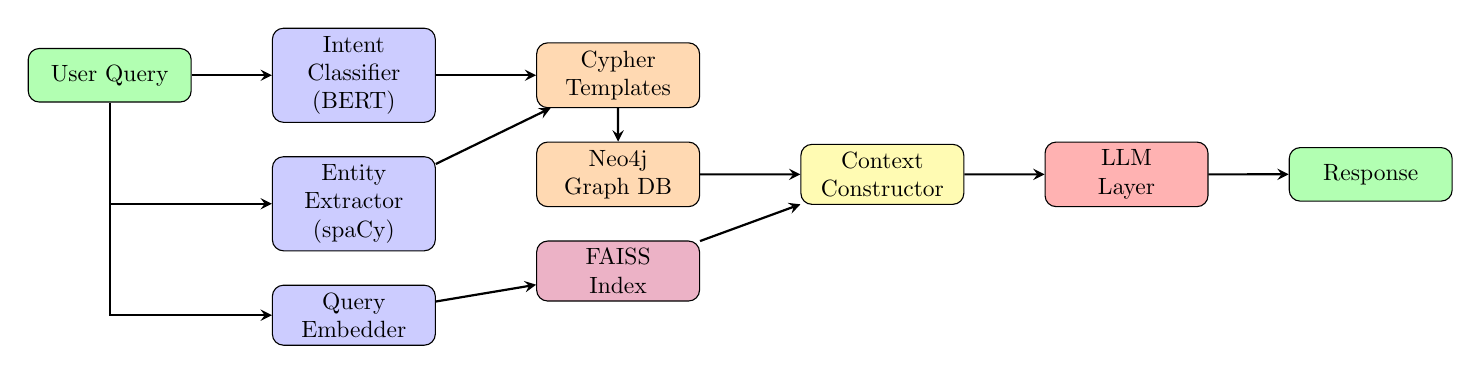
\begin{tikzpicture}[node distance=1.2cm, scale=0.85, transform shape,
    block/.style={rectangle, draw, fill=blue!20, text width=2.2cm, text centered, minimum height=0.8cm, rounded corners},
    arrow/.style={->, >=stealth, thick}]

    % Input
    \node[block, fill=green!30] (input) {User Query};

    % Preprocessing
    \node[block, right=of input] (intent) {Intent\\Classifier\\(BERT)};
    \node[block, below=0.5cm of intent] (entity) {Entity\\Extractor\\(spaCy)};
    \node[block, below=0.5cm of entity] (embed) {Query\\Embedder};

    % Retrieval
    \node[block, right=1.5cm of intent, fill=orange!30] (cypher) {Cypher\\Templates};
    \node[block, below=0.5cm of cypher, fill=orange!30] (neo4j) {Neo4j\\Graph DB};
    \node[block, below=0.5cm of neo4j, fill=purple!30] (faiss) {FAISS\\Index};

    % Context
    \node[block, right=1.5cm of neo4j, fill=yellow!30] (context) {Context\\Constructor};

    % LLM
    \node[block, right=of context, fill=red!30] (llm) {LLM\\Layer};

    % Output
    \node[block, right=of llm, fill=green!30] (output) {Response};

    % Arrows
    \draw[arrow] (input) -- (intent);
    \draw[arrow] (input) |- (entity);
    \draw[arrow] (input) |- (embed);
    \draw[arrow] (intent) -- (cypher);
    \draw[arrow] (entity) -- (cypher);
    \draw[arrow] (cypher) -- (neo4j);
    \draw[arrow] (embed) -- (faiss);
    \draw[arrow] (neo4j) -- (context);
    \draw[arrow] (faiss) -- (context);
    \draw[arrow] (context) -- (llm);
    \draw[arrow] (llm) -- (output);

\end{tikzpicture}
\end{center}

\vspace{0.3cm}
\textbf{Task:} Hotel Recommendation Chatbot

\textbf{Dataset:} Custom hotel reviews dataset (hotels, users, reviews)
\end{frame}

%==============================================================================
% SECTION 2: INPUT PREPROCESSING
%==============================================================================
\section{Input Preprocessing}

\begin{frame}{Intent Classification - Fine Tuning a BERT Model}
\begin{columns}
\begin{column}{0.5\textwidth}
\textbf{Model:} \texttt{bert-base-uncased}

\textbf{Dataset:} Custom labeled dataset (200 samples)
% \textbf{Training Config:}
% \begin{itemize}
%     \item Learning rate: 5e-5
%     \item Batch size: 16
%     \item Epochs: 15
%     \item Train/Test split: 85/15
% \end{itemize}

\vspace{0.3cm}
\textbf{10 Intent Classes:}
\begin{enumerate}
    \scriptsize
    \item hotel\_recommendation
    \item hotel\_search
    \item hotel\_info
    \item review\_query
    \item comparison
    \item traveller\_preference
    \item location\_query
    \item visa\_query
    \item rating\_filter
    \item general\_question
\end{enumerate}
\end{column}

\begin{column}{0.5\textwidth}
\textbf{Classification Examples:}

\vspace{0.2cm}
\begin{tabular}{|p{4cm}|l|}
\hline
\textbf{Query} & \textbf{Intent} \\
\hline
``Recommend me a hotel in Tokyo'' & hotel\_rec (0.97) \\
\hline
``Do I need visa from India?'' & visa\_query (0.89) \\
\hline
``Compare Azure Tower and Marina'' & comparison (0.94) \\
\hline
``Best for business travelers'' & traveller\_pref (0.91) \\
\hline
``Hotels with rating above 9'' & rating\_filter (0.88) \\
\hline
\end{tabular}
\end{column}
\end{columns}
\end{frame}

%------------------------------------------------------------------------------
\begin{frame}{Entity Extraction}
\begin{columns}
\begin{column}{0.45\textwidth}
\textbf{Approach:} Utiize NER library dataset keyword lookups

\vspace{0.2cm}
\textbf{Entity Types Extracted:}
\begin{itemize}
    \item \textbf{Hotels} - FAC, ORG labels + lookup
    \item \textbf{Cities/Countries} - GPE label
    \item \textbf{Traveller Types} - Lookup
    \item \textbf{Demographics (Gender + Age)} - Lookup + DATE lable
    \item \textbf{Ratings} - Lookup
\end{itemize}

\vspace{0.2cm}
\textbf{Keyword Example:}
\begin{itemize}
    \scriptsize
    \item solo, alone $\rightarrow$ ``Solo''
    \item business, corporate $\rightarrow$ ``Business''
    \item hygiene, cleanliness $\rightarrow$ cleanliness\_base
    \item senior, older $\rightarrow$ age\_group ``55+''
\end{itemize}
\end{column}

\begin{column}{0.55\textwidth}
\textbf{Extraction Examples:}

\vspace{0.2cm}
\footnotesize
\texttt{Query: ``Best hotels for solo female in Paris''}
\begin{itemize}
    \scriptsize
    \item cities: [``Paris'']
    \item traveller\_types: [``Solo'']
    \item demographics: [``Female'']
\end{itemize}

\vspace{0.2cm}
\texttt{Query: ``Hotels with cleanliness above 9''}
\begin{itemize}
    \scriptsize
    \item cleanliness\_base: 9.0
    \item comfort\_base: None
    \item facilities\_base: None
\end{itemize}

\vspace{0.2cm}
\texttt{Query: ``Compare Azure Tower and Marina Bay''}
\begin{itemize}
    \scriptsize
    \item hotels: [``The Azure Tower'', ``Marina Bay'']
\end{itemize}
\end{column}
\end{columns}
\end{frame}
%==============================================================================
%  ERROR ANALYSIS & IMPROVEMENTS
%==============================================================================
\section{Error Analysis \& Improvements}

\begin{frame}[t]{Error Analysis \& Limitations}
\vspace{0.2cm}
\textbf{Intent Classification:}
\begin{itemize}
    \setlength{\itemsep}{0.2em}
    \item Multi-intent queries not supported (``Find hotels and compare them'')
    \item Limited training data (200 generated samples)
    \item Out-of-domain queries classified with false confidence
    \item No intent hierarchy or fallback mechanism
\end{itemize}

\vspace{0.4cm}
\textbf{Entity Extraction:}
\begin{itemize}
    \setlength{\itemsep}{0.2em}
    \item Hotel names with special characters missed (L'Étoile)
    \item Some relies on predefined keyword lists (not adaptive)
    \item spaCy NER misses domain-specific entities
    \item No coreference resolution (``that hotel'')
\end{itemize}
\end{frame}
%------------------------------------------------------------------------------
\begin{frame}{Query Processing for Embeddings}
\begin{columns}
\begin{column}{0.5\textwidth}
\textbf{Query-to-Embedding Flow:}

\begin{enumerate}
    \item User query received
    \item Entity extraction (hotel names, cities)
    \item If hotel name found $\rightarrow$ similarity search
    \item Retrieve hotel's embedding from FAISS
    \item Find k-nearest neighbors
    \item Return ranked similar hotels
\end{enumerate}

\vspace{0.3cm}
\textbf{Fallback for No Hotel Name:}
\begin{itemize}
    \scriptsize
    \item Keyword matching on city/country
    \item Use first result from KG context
    \item Basic text similarity scoring
\end{itemize}
\end{column}

\begin{column}{0.5\textwidth}
\textbf{FAISS Similarity Search:}

\vspace{0.2cm}
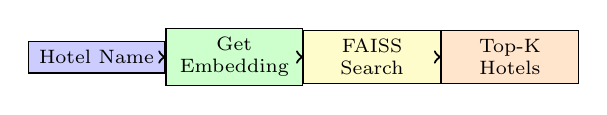
\begin{tikzpicture}[scale=0.7]
    \node[draw, rectangle, fill=blue!20, font=\scriptsize, text width=1.5cm, align=center] (q) at (0,0) {Hotel Name};
    \node[draw, rectangle, fill=green!20, font=\scriptsize, text width=1.5cm, align=center] (e) at (2.5,0) {Get Embedding};
    \node[draw, rectangle, fill=yellow!20, font=\scriptsize, text width=1.5cm, align=center] (m) at (5,0) {FAISS Search};
    \node[draw, rectangle, fill=orange!20, font=\scriptsize, text width=1.5cm, align=center] (f) at (7.5,0) {Top-K Hotels};
    \draw[->, thick] (q) -- (e);
    \draw[->, thick] (e) -- (m);
    \draw[->, thick] (m) -- (f);
\end{tikzpicture}

\vspace{0.3cm}
\textbf{Index Structure:}
\begin{itemize}
    \scriptsize
    \item Normalized L2 embeddings
    \item IndexFlatIP (Inner Product)
    \item Cosine similarity after normalization
    \item Separate index per model (Node2Vec/FastRP)
\end{itemize}

\vspace{0.2cm}
\textbf{Storage:}
\begin{itemize}
    \scriptsize
    \item Neo4j: node2vecEmbedding, fastRPEmbedding
    \item FAISS: faiss\_hotel\_index.bin, faiss\_hotel\_fastrp\_index.bin
\end{itemize}
\end{column}
\end{columns}
\end{frame}

%==============================================================================
% SECTION 3: GRAPH RETRIEVAL - BASELINE
%==============================================================================
\section{Graph Retrieval - Baseline}

\begin{frame}{Knowledge Graph Schema - Complete Overview}
\begin{columns}
\begin{column}{0.55\textwidth}
\textbf{Node Types \& Properties:}

\vspace{0.2cm}
\footnotesize
\begin{tabular}{|l|p{5cm}|}
\hline
\textbf{Node} & \textbf{Properties} \\
\hline
\textbf{Hotel} & hotel\_id, name, star\_rating, avg\_reviewer\_score, review\_count, avg\_cleanliness, avg\_comfort, avg\_facilities, avg\_location, avg\_staff, avg\_value \\
\hline
\textbf{City} & name \\
\hline
\textbf{Country} & name \\
\hline
\textbf{Review} & review\_id, text, date, score\_overall, score\_cleanliness, score\_comfort, score\_facilities, score\_location, score\_staff, score\_value \\
\hline
\textbf{Traveller} & traveller\_id, age\_group, gender, traveller\_type \\
\hline
\end{tabular}
\end{column}

\begin{column}{0.45\textwidth}
\textbf{Relationships (7 types):}

\vspace{0.2cm}
\footnotesize
\begin{tabular}{|l|l|}
\hline
\textbf{Relationship} & \textbf{Pattern} \\
\hline
LOCATED\_IN & Hotel $\rightarrow$ City \\
LOCATED\_IN & City $\rightarrow$ Country \\
REVIEWED & Review $\rightarrow$ Hotel \\
WROTE & Traveller $\rightarrow$ Review \\
STAYED\_AT & Traveller $\rightarrow$ Hotel \\
FROM\_COUNTRY & Traveller $\rightarrow$ Country \\
NEEDS\_VISA & Country $\rightarrow$ Country \\
\hline
\end{tabular}

\vspace{0.3cm}
\textbf{Graph Statistics:}
\begin{itemize}
    \scriptsize
    \item 25 Hotels across 25 Cities
    \item 24 Countries with visa relations
    \item 500+ Reviews with scores
    \item 500+ Travellers with demographics
\end{itemize}
\end{column}
\end{columns}

\vspace{0.2cm}
\textbf{Key Design:} Hotels enriched with computed averages from reviews for embedding features
\end{frame}

%------------------------------------------------------------------------------
\begin{frame}{Cypher Query Templates (1/2)}
\begin{columns}
\begin{column}{0.5\textwidth}
\textbf{Location Queries:}
\footnotesize

\vspace{0.1cm}
\texttt{-- Hotels in city}

\texttt{MATCH (h:Hotel)-[:LOCATED\_IN]->(c:City)}

\texttt{WHERE c.name = \$city}

\texttt{RETURN h.name, h.star\_rating}

\vspace{0.2cm}
\texttt{-- Top rated in country}

\texttt{MATCH (h:Hotel)-[:LOCATED\_IN]->(c:City)}

\texttt{~~~~~~-[:LOCATED\_IN]->(co:Country)}

\texttt{WHERE co.name = \$country}

\texttt{RETURN h.name ORDER BY h.star\_rating DESC}

\vspace{0.2cm}
\texttt{-- Cities with hotels}

\texttt{MATCH (h:Hotel)-[:LOCATED\_IN]->(c:City)}

\texttt{RETURN DISTINCT c.name, h.name}
\end{column}

\begin{column}{0.5\textwidth}
\textbf{Review Queries:}
\footnotesize

\vspace{0.1cm}
\texttt{-- Hotel reviews}

\texttt{MATCH (h:Hotel)<-[:REVIEWED]-(r:Review)}

\texttt{WHERE h.name = \$hotel\_name}

\texttt{RETURN r.text, r.score\_overall LIMIT 10}

\vspace{0.2cm}
\texttt{-- Reviews by demographic}

\texttt{MATCH (h:Hotel)<-[:REVIEWED]-(r:Review)}

\texttt{~~~~~~<-[:WROTE]-(t:Traveller)}

\texttt{WHERE h.name = \$hotel\_name}

\texttt{~~AND t.gender = \$gender}

\texttt{RETURN r.text, r.score\_overall}
\end{column}
\end{columns}
\end{frame}

%------------------------------------------------------------------------------
\begin{frame}{Cypher Query Templates (2/2)}
\begin{columns}
\begin{column}{0.5\textwidth}
\textbf{Visa \& Traveller Queries:}
\footnotesize

\vspace{0.1cm}
\texttt{-- Countries requiring visa}

\texttt{MATCH (tc:Country)-[:NEEDS\_VISA]->(co:Country)}

\texttt{WHERE tc.name = \$from\_country}

\texttt{RETURN co.name}

\vspace{0.2cm}
\texttt{-- Hotels without visa needed}

\texttt{MATCH (tc:Country), (h:Hotel)-[:LOCATED\_IN]}

\texttt{~~~~~~->(c:City)-[:LOCATED\_IN]->(co:Country)}

\texttt{WHERE tc.name = \$from AND NOT}

\texttt{~~~~~~(tc)-[:NEEDS\_VISA]->(co)}

\texttt{RETURN DISTINCT h.name}

\vspace{0.2cm}
\texttt{-- Best for traveller type}

\texttt{MATCH (h:Hotel)<-[:REVIEWED]-(r:Review)}

\texttt{~~~~~~<-[:WROTE]-(t:Traveller)}

\texttt{WHERE t.type = \$type}

\texttt{RETURN h.name, AVG(r.score\_overall)}
\end{column}

\begin{column}{0.5\textwidth}
\textbf{Rating \& Comparison:}
\footnotesize

\vspace{0.1cm}
\texttt{-- Hotels by cleanliness}

\texttt{MATCH (h:Hotel)}

\texttt{WHERE h.cleanliness\_base >= \$min}

\texttt{RETURN h.name, h.cleanliness\_base}

\texttt{ORDER BY h.cleanliness\_base DESC}

\vspace{0.2cm}
\texttt{-- Compare two hotels}

\texttt{MATCH (h1:Hotel), (h2:Hotel)}

\texttt{WHERE h1.name = \$hotel1}

\texttt{~~AND h2.name = \$hotel2}

\texttt{RETURN h1, h2}

\vspace{0.2cm}
\texttt{-- Hotels with most reviews}

\texttt{MATCH (h:Hotel)<-[:REVIEWED]-(r:Review)}

\texttt{RETURN h.name, COUNT(r) as cnt}

\texttt{ORDER BY cnt DESC LIMIT \$top\_n}

\vspace{0.3cm}
\textbf{Total: 31 Cypher Templates}
\end{column}
\end{columns}
\end{frame}

%------------------------------------------------------------------------------
\begin{frame}{Retrieved Data Examples}
\textbf{Query:} ``Recommend me a hotel in Tokyo''

\begin{columns}
\begin{column}{0.5\textwidth}
\textbf{Pipeline Output:}
\begin{itemize}
    \item Intent: hotel\_recommendation
    \item Entities: cities=[``Tokyo''], countries=[``Japan'']
\end{itemize}

\vspace{0.2cm}
\textbf{Cypher Results:}

\footnotesize
\begin{tabular}{|l|c|l|}
\hline
\textbf{Hotel} & \textbf{Rating} & \textbf{City} \\
\hline
The Azure Tower & 4.8 & Tokyo \\
Sakura Grand Hotel & 4.6 & Tokyo \\
Imperial Garden Inn & 4.5 & Tokyo \\
\hline
\end{tabular}
\end{column}

\begin{column}{0.5\textwidth}
\textbf{Query:} ``Best for business travelers''

\vspace{0.2cm}
\textbf{Pipeline Output:}
\begin{itemize}
    \item Intent: traveller\_preference
    \item Entities: traveller\_types=[``Business'']
\end{itemize}

\vspace{0.2cm}
\textbf{Cypher Results:}

\footnotesize
\begin{tabular}{|l|c|}
\hline
\textbf{Hotel} & \textbf{Avg Score} \\
\hline
Executive Suites & 9.2 \\
Business Bay Hotel & 8.9 \\
Corporate Tower & 8.7 \\
\hline
\end{tabular}
\end{column}
\end{columns}
\end{frame}

%==============================================================================
% SECTION 4: EMBEDDING-BASED RETRIEVAL
%==============================================================================
\section{Embedding-Based Retrieval}

\begin{frame}{Dual Node Embedding Approach}
\begin{center}
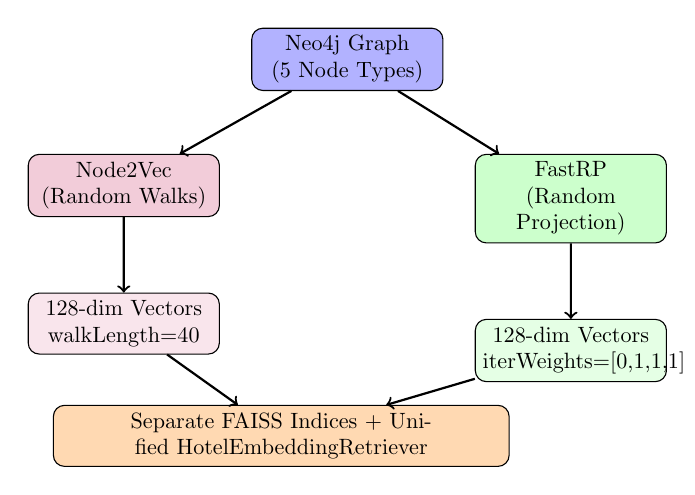
\begin{tikzpicture}[node distance=1.2cm, scale=0.8, transform shape,
    block/.style={rectangle, draw, fill=blue!20, text width=2.8cm, text centered, minimum height=0.9cm, rounded corners}]

    % Shared graph input
    \node[block, fill=blue!30] (graph) {Neo4j Graph\\(5 Node Types)};

    % Left side - Node2Vec
    \node[block, below left=1cm and 0.5cm of graph, fill=purple!20] (n2v) {Node2Vec\\(Random Walks)};
    \node[block, below=of n2v, fill=purple!10] (n2vemb) {128-dim Vectors\\walkLength=40};

    % Right side - FastRP
    \node[block, below right=1cm and 0.5cm of graph, fill=green!20] (frp) {FastRP\\(Random Projection)};
    \node[block, below=of frp, fill=green!10] (frpemb) {128-dim Vectors\\iterWeights=[0,1,1,1]};

    % FAISS
    \node[block, below=0.8cm of n2vemb, fill=orange!30, text width=7cm, xshift=2.5cm] (faiss) {Separate FAISS Indices + Unified HotelEmbeddingRetriever};

    % Arrows
    \draw[->, thick] (graph) -- (n2v);
    \draw[->, thick] (graph) -- (frp);
    \draw[->, thick] (n2v) -- (n2vemb);
    \draw[->, thick] (frp) -- (frpemb);
    \draw[->, thick] (n2vemb) -- (faiss);
    \draw[->, thick] (frpemb) -- (faiss);

\end{tikzpicture}
\end{center}

\vspace{0.2cm}
\textbf{Approach:} Node Embeddings using two different graph algorithms from Neo4j GDS

\textbf{Requirement:} ``Choose ONE approach, experiment with at least TWO different embedding models''
\end{frame}

%------------------------------------------------------------------------------
\begin{frame}{Embedding Implementation Details}
\begin{columns}
\begin{column}{0.5\textwidth}
\textbf{Node2Vec (Random Walks):}
\begin{itemize}
    \scriptsize
    \item Uses Neo4j Graph Data Science (GDS)
    \item Random walks explore graph topology
    \item Parameters: walkLength=40, iterations=10
    \item Learns from node connectivity patterns
    \item All 5 node types embedded together
\end{itemize}

\vspace{0.2cm}
\textbf{How it works:}
\begin{enumerate}
    \scriptsize
    \item Project graph to GDS catalog
    \item Run gds.node2vec.write() algorithm
    \item Extract 128-dim vectors per node
    \item Build FAISS index for hotels only
    \item Store in Neo4j vector index
\end{enumerate}
\end{column}

\begin{column}{0.5\textwidth}
\textbf{FastRP (Random Projection):}
\begin{itemize}
    \scriptsize
    \item Also uses Neo4j GDS library
    \item Random projection-based embeddings
    \item Parameters: iterationWeights=[0,1,1,1]
    \item Faster computation than Node2Vec
    \item Same graph structure input
\end{itemize}

\vspace{0.2cm}
\textbf{How it works:}
\begin{enumerate}
    \scriptsize
    \item Project graph to GDS catalog
    \item Run gds.fastRP.write() algorithm
    \item Extract 128-dim vectors per node
    \item Build separate FAISS index
    \item Store in Neo4j vector index
\end{enumerate}

\vspace{0.2cm}
\textbf{Key Difference:}
\begin{itemize}
    \scriptsize
    \item Node2Vec: Simulates walks (slower, more expressive)
    \item FastRP: Random projections (faster, efficient)
\end{itemize}
\end{column}
\end{columns}
\end{frame}

%------------------------------------------------------------------------------
\begin{frame}{Embedding Models Comparison}
\begin{table}
\centering
\footnotesize
\begin{tabular}{lcc}
\toprule
\textbf{Property} & \textbf{Node2Vec} & \textbf{FastRP} \\
\midrule
Algorithm & Random Walks & Random Projection \\
Dimension & 128 & 128 \\
Neo4j GDS Function & gds.node2vec.write() & gds.fastRP.write() \\
Input & Graph structure (5 node types) & Graph structure (5 node types) \\
\midrule
Walk Length & 40 & -- \\
Iterations & 10 & -- \\
Iteration Weights & -- & [0.0, 1.0, 1.0, 1.0] \\
Computation Time & $\sim$2-3s & $\sim$0.2s \\
\midrule
Storage & Neo4j + FAISS & Neo4j + FAISS \\
Similarity & Cosine (via FAISS) & Cosine (via FAISS) \\
\bottomrule
\end{tabular}
\caption{Two Node Embedding Models for Comparison}
\end{table}

\vspace{0.2cm}
\begin{columns}
\begin{column}{0.5\textwidth}
\textbf{Node2Vec Strengths:}
\begin{itemize}
    \scriptsize
    \item Captures higher-order neighborhood patterns
    \item Better at finding structurally similar nodes
    \item Flexible p,q parameters for exploration
    \item More expressive representations
\end{itemize}
\end{column}
\begin{column}{0.5\textwidth}
\textbf{FastRP Strengths:}
\begin{itemize}
    \scriptsize
    \item 10x faster computation ($\sim$0.2s vs $\sim$2s)
    \item Memory efficient
    \item Good for large-scale graphs
    \item Simpler hyperparameters
\end{itemize}
\end{column}
\end{columns}
\end{frame}

%------------------------------------------------------------------------------
\begin{frame}{Embedding Retrieval Results - Similar Hotels}
\begin{columns}
\begin{column}{0.5\textwidth}
\textbf{Node2Vec Search:}

Query Hotel: ``Berlin Mitte Elite''

\vspace{0.2cm}
\footnotesize
\begin{tabular}{|l|c|}
\hline
\textbf{Similar Hotel} & \textbf{Score} \\
\hline
Colosseum Gardens (Rome) & 0.686 \\
Aztec Heights (Mexico City) & 0.663 \\
Table Mountain View (Cape Town) & 0.587 \\
\hline
\end{tabular}

\vspace{0.2cm}
\textbf{Method:} Random walks capture neighborhood structure and traveller patterns
\end{column}

\begin{column}{0.5\textwidth}
\textbf{FastRP Search:}

Query Hotel: ``Berlin Mitte Elite''

\vspace{0.2cm}
\footnotesize
\begin{tabular}{|l|c|}
\hline
\textbf{Similar Hotel} & \textbf{Score} \\
\hline
The Kiwi Grand (Wellington) & 0.712 \\
Han River Oasis (Seoul) & 0.698 \\
Kremlin Suites (Moscow) & 0.685 \\
\hline
\end{tabular}

\vspace{0.2cm}
\textbf{Method:} Random projections capture immediate neighborhood relationships
\end{column}
\end{columns}

\vspace{0.3cm}
\textbf{Key Insight:} Both capture graph structure, but Node2Vec explores deeper paths while FastRP focuses on immediate neighbors.
\end{frame}

%------------------------------------------------------------------------------
\begin{frame}{Embedding Comparison in UI}
\begin{columns}
\begin{column}{0.5\textwidth}
\textbf{Side-by-Side Comparison:}

\vspace{0.2cm}
The UI displays results from both embedding models simultaneously when a hotel is mentioned or found in context.

\vspace{0.3cm}
\textbf{Example Query:} ``Tell me about The Azure Tower''

\vspace{0.2cm}
\footnotesize
\begin{tabular}{|l|c|}
\hline
\multicolumn{2}{|c|}{\textbf{Node2Vec Results}} \\
\hline
Colosseum Gardens & 0.739 \\
Tango Suites & 0.710 \\
The Royal Compass & 0.693 \\
\hline
\end{tabular}

\vspace{0.2cm}
\begin{tabular}{|l|c|}
\hline
\multicolumn{2}{|c|}{\textbf{FastRP Results}} \\
\hline
Gaudi's Retreat & 0.583 \\
Marina Bay Zenith & 0.567 \\
The Golden Oasis & 0.553 \\
\hline
\end{tabular}
\end{column}

\begin{column}{0.5\textwidth}
\textbf{Why Different Results?}

\vspace{0.2cm}
\begin{itemize}
    \scriptsize
    \item \textbf{Node2Vec:} Explores deeper graph paths via random walks
    \item \textbf{FastRP:} Captures immediate neighborhood via projections
    \item Same hotel can have different ``similar'' hotels
    \item Validates both models work independently
\end{itemize}

\vspace{0.3cm}
\textbf{UI Features:}
\begin{itemize}
    \scriptsize
    \item Automatic hotel extraction from query
    \item Falls back to first hotel in KG context
    \item Shows rank and similarity score
    \item Helps evaluate embedding quality
\end{itemize}

\vspace{0.2cm}
\textbf{Selected Model:} Sidebar dropdown chooses which embedding feeds into LLM context
\end{column}
\end{columns}
\end{frame}

%------------------------------------------------------------------------------
\begin{frame}{Embedding Models - Quantitative Comparison}
\begin{table}
\centering
\begin{tabular}{lccc}
\toprule
\textbf{Metric} & \textbf{Node2Vec} & \textbf{FastRP} & \textbf{Notes} \\
\midrule
Embedding Dimension & 128 & 128 & Same dimensionality \\
Algorithm & Random Walks & Random Projection & Different approaches \\
Setup Time & $\sim$2-3s & $\sim$0.2s & FastRP 10x faster \\
Query Latency & 2-4ms & 2-4ms & Similar (FAISS) \\
\midrule
GDS Function & gds.node2vec.write() & gds.fastRP.write() & Neo4j GDS \\
Key Parameters & walkLength, iterations & iterationWeights & Tunable \\
Memory Usage & Higher & Lower & FastRP more efficient \\
\bottomrule
\end{tabular}
\caption{Node2Vec vs FastRP Performance Comparison}
\end{table}

\vspace{0.2cm}
\textbf{Key Differences:}
\begin{itemize}
    \scriptsize
    \item \textbf{Node2Vec}: Captures higher-order neighborhood patterns through simulated walks
    \item \textbf{FastRP}: Faster computation, good for large graphs, simpler hyperparameters
    \item \textbf{Results}: Different similar hotels returned (as shown in UI comparison)
    \item \textbf{Unified Interface}: HotelEmbeddingRetriever allows runtime model switching
\end{itemize}
\end{frame}

%------------------------------------------------------------------------------
\begin{frame}{Unified Retriever Interface}
\textbf{Black-Box Design Pattern:} Single interface abstracts both embedding models

\vspace{0.3cm}
\begin{columns}
\begin{column}{0.5\textwidth}
\textbf{Simple Function API:}
\footnotesize

\texttt{from embeddings\_retreiver import}

\texttt{~~~~search\_hotels, set\_model\_type}

\vspace{0.2cm}
\texttt{\# Default: node2vec model}

\texttt{results = search\_hotels("hotel in Paris")}

\vspace{0.2cm}
\texttt{\# Switch to fastrp}

\texttt{set\_model\_type('fastrp')}

\texttt{results = search\_hotels("beach hotel")}
\end{column}

\begin{column}{0.5\textwidth}
\textbf{Class API (more control):}
\footnotesize

\texttt{retriever = HotelEmbeddingRetriever(}

\texttt{~~~~driver, model\_type='node2vec')}

\vspace{0.2cm}
\texttt{\# Same methods for both models}

\texttt{retriever.find\_similar\_hotels(name)}

\texttt{retriever.search\_by\_query(query)}

\vspace{0.2cm}
\texttt{\# Runtime model switching}

\texttt{retriever.model\_type = 'fastrp'}
\end{column}
\end{columns}

\vspace{0.3cm}
\textbf{Auto-initialization:} Loads existing FAISS index or runs setup if needed
\end{frame}

%==============================================================================
% SECTION 5: LLM LAYER
%==============================================================================
\section{LLM Layer}

\begin{frame}{Context Construction}
\textbf{Process Flow:}

\begin{enumerate}
    \item \textbf{Intent Classification} $\rightarrow$ Select relevant Cypher templates
    \item \textbf{Entity Extraction} $\rightarrow$ Fill template parameters
    \item \textbf{Graph Retrieval} $\rightarrow$ Execute Cypher queries on Neo4j
    \item \textbf{Embedding Retrieval} $\rightarrow$ FAISS similarity search
    \item \textbf{Context Merge} $\rightarrow$ Combine all results
\end{enumerate}

\vspace{0.3cm}
\textbf{Intent-based Query Selection:}

\footnotesize
\begin{tabular}{|l|l|}
\hline
\textbf{Intent} & \textbf{Cypher Queries Used} \\
\hline
hotel\_recommendation & get\_top\_rated\_hotels\_in\_city, get\_top\_rated\_hotels\_in\_country \\
\hline
visa\_query & get\_countries\_requiring\_visa, get\_hotels\_accessible\_without\_visa \\
\hline
traveller\_preference & get\_best\_hotels\_for\_traveller\_type, get\_best\_hotels\_for\_gender \\
\hline
comparison & compare\_two\_hotels \\
\hline
\end{tabular}
\end{frame}

%------------------------------------------------------------------------------
\begin{frame}{Prompt Structure}
\textbf{Persona Definition:}

\footnotesize
``You are J.A.R.V.I.S., an advanced AI hotel concierge assistant. You speak with sophisticated eloquence and always address the user as 'sir' or 'madam'. Your responses are warm yet professional, helpful and conversational - never robotic or formulaic.''

\vspace{0.3cm}
\normalsize
\textbf{Key Instructions:}

\footnotesize
\begin{itemize}
    \item Address the user respectfully as ``sir'' at least once
    \item NEVER start with ``Based on the data provided'' or similar phrases
    \item Be conversational and natural, like having a pleasant discussion
    \item Provide specific details without mentioning ``the data'' or ``the context''
    \item Explain WHY hotels would be good choices
    \item Keep responses concise but informative
\end{itemize}

\vspace{0.3cm}
\normalsize
\textbf{Context Injection:}

\footnotesize
Hotel information from KG retrieval and embedding search is appended to the prompt, but the LLM is instructed to present it naturally without referencing it as ``data''.
\end{frame}

%------------------------------------------------------------------------------
\begin{frame}{LLM Comparison - Models}
\begin{table}
\centering
\begin{tabular}{lccc}
\toprule
\textbf{Property} & \textbf{Gemma-2-2B} & \textbf{Mistral-7B} & \textbf{LLaMA-3.1-8B} \\
\midrule
Parameters & 2B & 7B & 8B \\
Provider & Google & Mistral AI & Meta \\
API & HuggingFace & HuggingFace & HuggingFace \\
Temperature & 0.2 & 0.2 & 0.2 \\
Max Tokens & 500 & 500 & 500 \\
\bottomrule
\end{tabular}
\end{table}

\vspace{0.3cm}
\textbf{Integration:} LangChain wrappers for HuggingFace Inference API

\vspace{0.2cm}
\textbf{Wrapper Pattern:}
\begin{itemize}
    \footnotesize
    \item Custom LLM class extending LangChain base
    \item Chat completion with message formatting
    \item Configurable max\_tokens and temperature
\end{itemize}
\end{frame}

%------------------------------------------------------------------------------
\begin{frame}{LLM Comparison - Quantitative Results}
\begin{table}
\centering
\begin{tabular}{lccccc}
\toprule
\textbf{Model} & \textbf{Latency (s)} & \textbf{Input Tok} & \textbf{Output Tok} & \textbf{Cost (\$)} & \textbf{Sem. Acc.} \\
\midrule
Gemma-2-2B & 1.2 & 45 & 150 & 0.00004 & 0.78 \\
Mistral-7B & 2.1 & 45 & 180 & 0.00012 & 0.84 \\
LLaMA-3.1-8B & 2.8 & 45 & 200 & 0.00018 & 0.86 \\
\bottomrule
\end{tabular}
\caption{Performance Metrics (averaged across test queries)}
\end{table}

\vspace{0.3cm}
\textbf{Semantic Accuracy Calculation:}

Cosine similarity between LLM response embedding and reference answer embedding using SentenceTransformer (all-MiniLM-L6-v2).

\vspace{0.2cm}
\textbf{Cost Calculation:} Based on HuggingFace API pricing per 1K tokens.
\end{frame}

%------------------------------------------------------------------------------
\begin{frame}{LLM Comparison - Qualitative Evaluation}
\begin{columns}
\begin{column}{0.33\textwidth}
\textbf{Gemma-2-2B}
\begin{itemize}
    \scriptsize
    \item Fastest response
    \item Concise answers
    \item Sometimes incomplete
    \item Good for simple queries
\end{itemize}
\end{column}

\begin{column}{0.33\textwidth}
\textbf{Mistral-7B}
\begin{itemize}
    \scriptsize
    \item Balanced performance
    \item Good reasoning
    \item Handles complex queries
    \item Best cost/quality ratio
\end{itemize}
\end{column}

\begin{column}{0.33\textwidth}
\textbf{LLaMA-3.1-8B}
\begin{itemize}
    \scriptsize
    \item Most detailed
    \item Best accuracy
    \item Higher latency
    \item Best for complex tasks
\end{itemize}
\end{column}
\end{columns}

\vspace{0.5cm}
\begin{center}
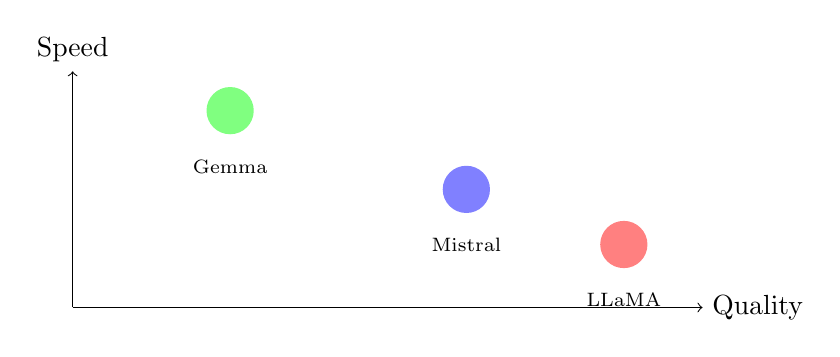
\begin{tikzpicture}
    \draw[->] (0,0) -- (8,0) node[right] {Quality};
    \draw[->] (0,0) -- (0,3) node[above] {Speed};

    \node[circle, fill=green!50, minimum size=0.6cm] at (2,2.5) {};
    \node[below] at (2,2) {\scriptsize Gemma};

    \node[circle, fill=blue!50, minimum size=0.6cm] at (5,1.5) {};
    \node[below] at (5,1) {\scriptsize Mistral};

    \node[circle, fill=red!50, minimum size=0.6cm] at (7,0.8) {};
    \node[below] at (7,0.3) {\scriptsize LLaMA};
\end{tikzpicture}
\end{center}
\end{frame}



%==============================================================================
% SECTION 7: LIVE DEMO
%==============================================================================
\section{Live Demo}

\begin{frame}{Pipeline Recap for Demo}
\begin{center}
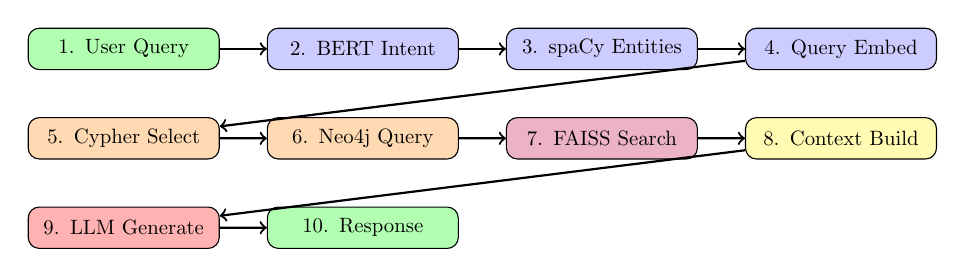
\begin{tikzpicture}[node distance=0.8cm, scale=0.75, transform shape,
    pstep/.style={rectangle, draw, fill=blue!20, text width=3cm, text centered, minimum height=0.7cm, rounded corners}]

    \node[pstep, fill=green!30] (s1) {1. User Query};
    \node[pstep, right=of s1] (s2) {2. BERT Intent};
    \node[pstep, right=of s2] (s3) {3. spaCy Entities};
    \node[pstep, right=of s3] (s4) {4. Query Embed};

    \node[pstep, below=0.8cm of s1, fill=orange!30] (s5) {5. Cypher Select};
    \node[pstep, right=of s5, fill=orange!30] (s6) {6. Neo4j Query};
    \node[pstep, right=of s6, fill=purple!30] (s7) {7. FAISS Search};
    \node[pstep, right=of s7, fill=yellow!30] (s8) {8. Context Build};

    \node[pstep, below=0.8cm of s5, fill=red!30] (s9) {9. LLM Generate};
    \node[pstep, right=of s9, fill=green!30] (s10) {10. Response};

    \draw[->, thick] (s1) -- (s2);
    \draw[->, thick] (s2) -- (s3);
    \draw[->, thick] (s3) -- (s4);
    \draw[->, thick] (s4) -- (s5);
    \draw[->, thick] (s5) -- (s6);
    \draw[->, thick] (s6) -- (s7);
    \draw[->, thick] (s7) -- (s8);
    \draw[->, thick] (s8) -- (s9);
    \draw[->, thick] (s9) -- (s10);

\end{tikzpicture}
\end{center}

\vspace{0.3cm}
\textbf{Demo Features:}
\begin{itemize}
    \item Switch between embedding models (Node2Vec / FastRP)
    \item Switch between LLMs (Gemma / Mistral / LLaMA)
    \item Side-by-side embedding comparison
    \item Streamlit UI with J.A.R.V.I.S. persona
\end{itemize}
\end{frame}

%------------------------------------------------------------------------------
\begin{frame}{Demo Queries}
\textbf{Test Queries for Live Demo (Pre-loaded in UI):}

\begin{enumerate}
    \item \textbf{Recommendation:} ``Recommend me a good hotel in Tokyo''

    \item \textbf{Search:} ``Find hotels in Paris''

    \item \textbf{Hotel Info:} ``Tell me about The Azure Tower''

    \item \textbf{Reviews:} ``Show me reviews for The Golden Oasis''

    \item \textbf{Comparison:} ``Compare The Azure Tower and L'Etoile Palace''

    \item \textbf{Traveller:} ``Best hotels for business travelers''

    \item \textbf{Rating Filter:} ``Hotels with cleanliness rating above 9''

    \item \textbf{Demographics:} ``Hotels recommended for seniors''
\end{enumerate}

\vspace{0.3cm}
\begin{center}
\textbf{[LIVE DEMO]}
\end{center}
\end{frame}

%==============================================================================
\begin{frame}
\begin{center}
\Huge Thank You!

\vspace{1cm}
\Large Questions?
\end{center}
\end{frame}

\end{document}
